This section is new in this report. It asks what the final model looks at and what it uses (script \texttt{fr\_attention.py}, seed 0 of each link, 20{,}000 test windows per link). Attention weights show where the decoder looks. Input gradients show which inputs change the forecast. The two need not agree, and here they do not.

\begin{figure}[H]
  \centering
  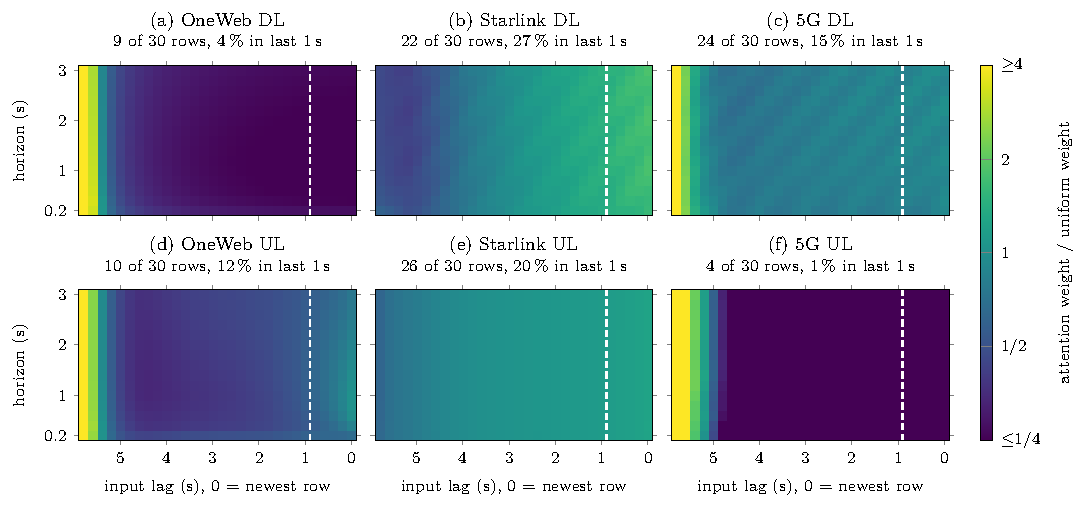
\includegraphics[width=\linewidth]{figs_pdf/fr_attention.pdf}
  \caption{Where the DS2S decoder looks in the 6\,s input window: mean attention over test windows for each input row (x, newest on the right) and forecast step (y), relative to uniform attention (1/30). Subtitles: effective number of rows read and share of attention on the last second (right of the white dashed line, 17\% if uniform).}
  \label{fig:attn}
\end{figure}

\begin{figure}[H]
  \centering
  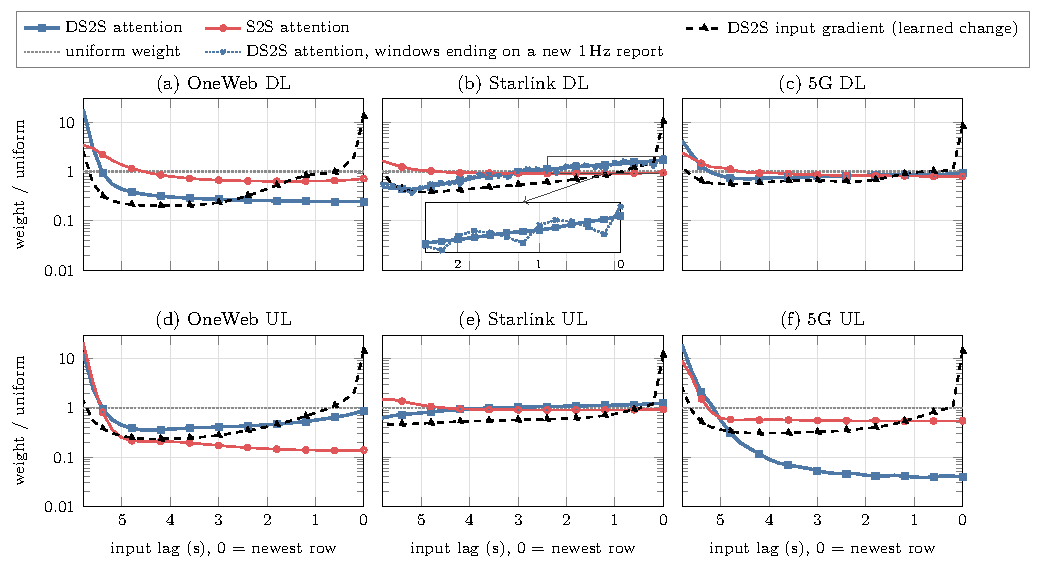
\includegraphics[width=\linewidth]{figs_pdf/fr_attention_prof.pdf}
  \caption{Attention of DS2S and S2S and the input gradient of the learned change of DS2S per input lag, relative to uniform weight (log scale). Inset (Starlink DL): attention in windows that end on a new 1\,Hz iperf report.}
  \label{fig:attnprof}
\end{figure}

\paragraph{What DS2S uses.} On every link the forecast is most sensitive to the newest second of input, which receives \GradLastLo\% to \GradLastHi\% of the input gradient of the learned change (17\% if uniform). A large share of the sensitivity at the 3\,s step, \GradEngLo\% to \GradEngHi\%, goes to the engineered trailing statistics (30 to 60\,s means and the session mean). These give DS2S a memory longer than its 6\,s window and let it read the regime of the session, which Section~\ref{sec:predictable} identified as the predictable part of the spread.

\paragraph{What DS2S looks at.} The attention mostly looks elsewhere (Fig.~\ref{fig:attn}). On OneWeb and 5G UL it puts \AttnSinkLo\% to \AttnSinkHi\% of its weight on the oldest encoder state, an attention sink, and on Starlink UL and 5G DL it is nearly flat. Recent inputs reach the forecast through the final encoder state, which starts the decoder, and through the last observed values that the anchored decoder adds its output to. On Starlink DL, where the iperf reports arrive once per second and are held for five rows, the attention locks onto report arrivals (Fig.~\ref{fig:attnprof}, inset).

\paragraph{Does attention matter?} Replacing the attention of every window by a fixed map learned on the calibration sessions, or by uniform weights, raises the RTT MAE by at most \AttnAblMax\% on Starlink and 5G. Attention matters only on OneWeb: uniform weights cost $+$\AttnAblOWDL\% on OneWeb DL and a fixed map $+$\AttnAblOWULmap\% on OneWeb UL. The attention maps describe what DS2S learned about the timing of the data, not why it is accurate. The gain of DS2S comes from its distributional output and its inputs, not from where it attends.
